\let\negmedspace\undefined
\let\negthickspace\undefined
\documentclass[journal]{IEEEtran}
\usepackage[a5paper, margin=10mm, onecolumn]{geometry}

\usepackage{tfrupee} 
\setlength{\headheight}{1cm} 
\setlength{\headsep}{0mm}       

\usepackage{gvv-book}
\usepackage{gvv}
\usepackage{cite}
\usepackage{amsmath,amssymb,amsfonts,amsthm}
\usepackage{algorithmic}
\usepackage{graphicx}
\usepackage{textcomp}
\usepackage{xcolor}
\usepackage{txfonts}
\usepackage{listings}
\usepackage{enumitem}
\usepackage{mathtools}
\usepackage{gensymb}
\usepackage{comment}
\usepackage[breaklinks=true]{hyperref}
\usepackage{tkz-euclide} 
\usepackage{listings}

\def\inputGnumericTable{}                                 
\usepackage[latin1]{inputenc}                                
\usepackage{color}                                            
\usepackage{array}                                            
\usepackage{longtable}                                       
\usepackage{calc}                                             
\usepackage{multirow}                                         
\usepackage{hhline}                                           
\usepackage{ifthen}                                           
\usepackage{lscape}

\begin{document}
	
	\bibliographystyle{IEEEtran}
	\vspace{3cm}
	
	\title{4.11.30}
	\author{EE25BTECH11052 - Shriyansh Kalpesh Chawda}
	{\let\newpage\relax\maketitle}
	
	
	\renewcommand{\thefigure}{\arabic{figure}}
	\renewcommand{\thetable}{\arabic{table}}
	\numberwithin{equation}{section} 
	\setcounter{section}{0}          
	\renewcommand{\theequation}{\arabic{equation}}
	
	\textbf{Question}:\\
	Draw the graph of the equations $x - y + 1 = 0$ and $3x + 2y - 12 = 0$. Using this graph, find the values of $x$ and $y$ which satisfy both the equations. 
	\hfill (10, 2021)
	
	\textbf{Solution.}\\
	Below is the Graph plotted for the given two lines. \\
	The lines intersect at $(2,3)$.\\
	The following is the solution using \textbf{Matrices and row Reduction}.\\
	\begin{enumerate}[label=(\roman*)]
		\item $x - y + 1 = 0 \;\Longrightarrow\; x - y = -1$
		\item $3x + 2y - 12 = 0 \;\Longrightarrow\; 3x + 2y = 12$
	\end{enumerate}
	
	Thus,
	\begin{align}
		\myvec{1 & -1 \\ 3 & 2}\vec{x} &= \myvec{-1 \\ 12}
	\end{align}
	
	Apply row reduction:
	\begin{align}
		R_2 &\to R_2 - 3R_1 \\
		\myvec{1 & -1 \\ 0 & 5}\vec{x} &= \myvec{-1 \\ 15}
	\end{align}
	
	\begin{align}
	R_2 &\to \tfrac{1}{5}R_2 \\
		\myvec{1 & -1 \\ 0 & 1}\vec{x} &= \myvec{-1 \\ 3}
	\end{align}
	
	\begin{align}
	R_1 &\to R_1 + R_2 \\
		\myvec{1 & 0 \\ 0 & 1}\vec{x} &= \myvec{2 \\ 3}
	\end{align}
	
	\begin{align}
		\therefore \; \vec{x} = \myvec{2 \\ 3}
	\end{align}
	
	\begin{figure}[H]
		\centering
		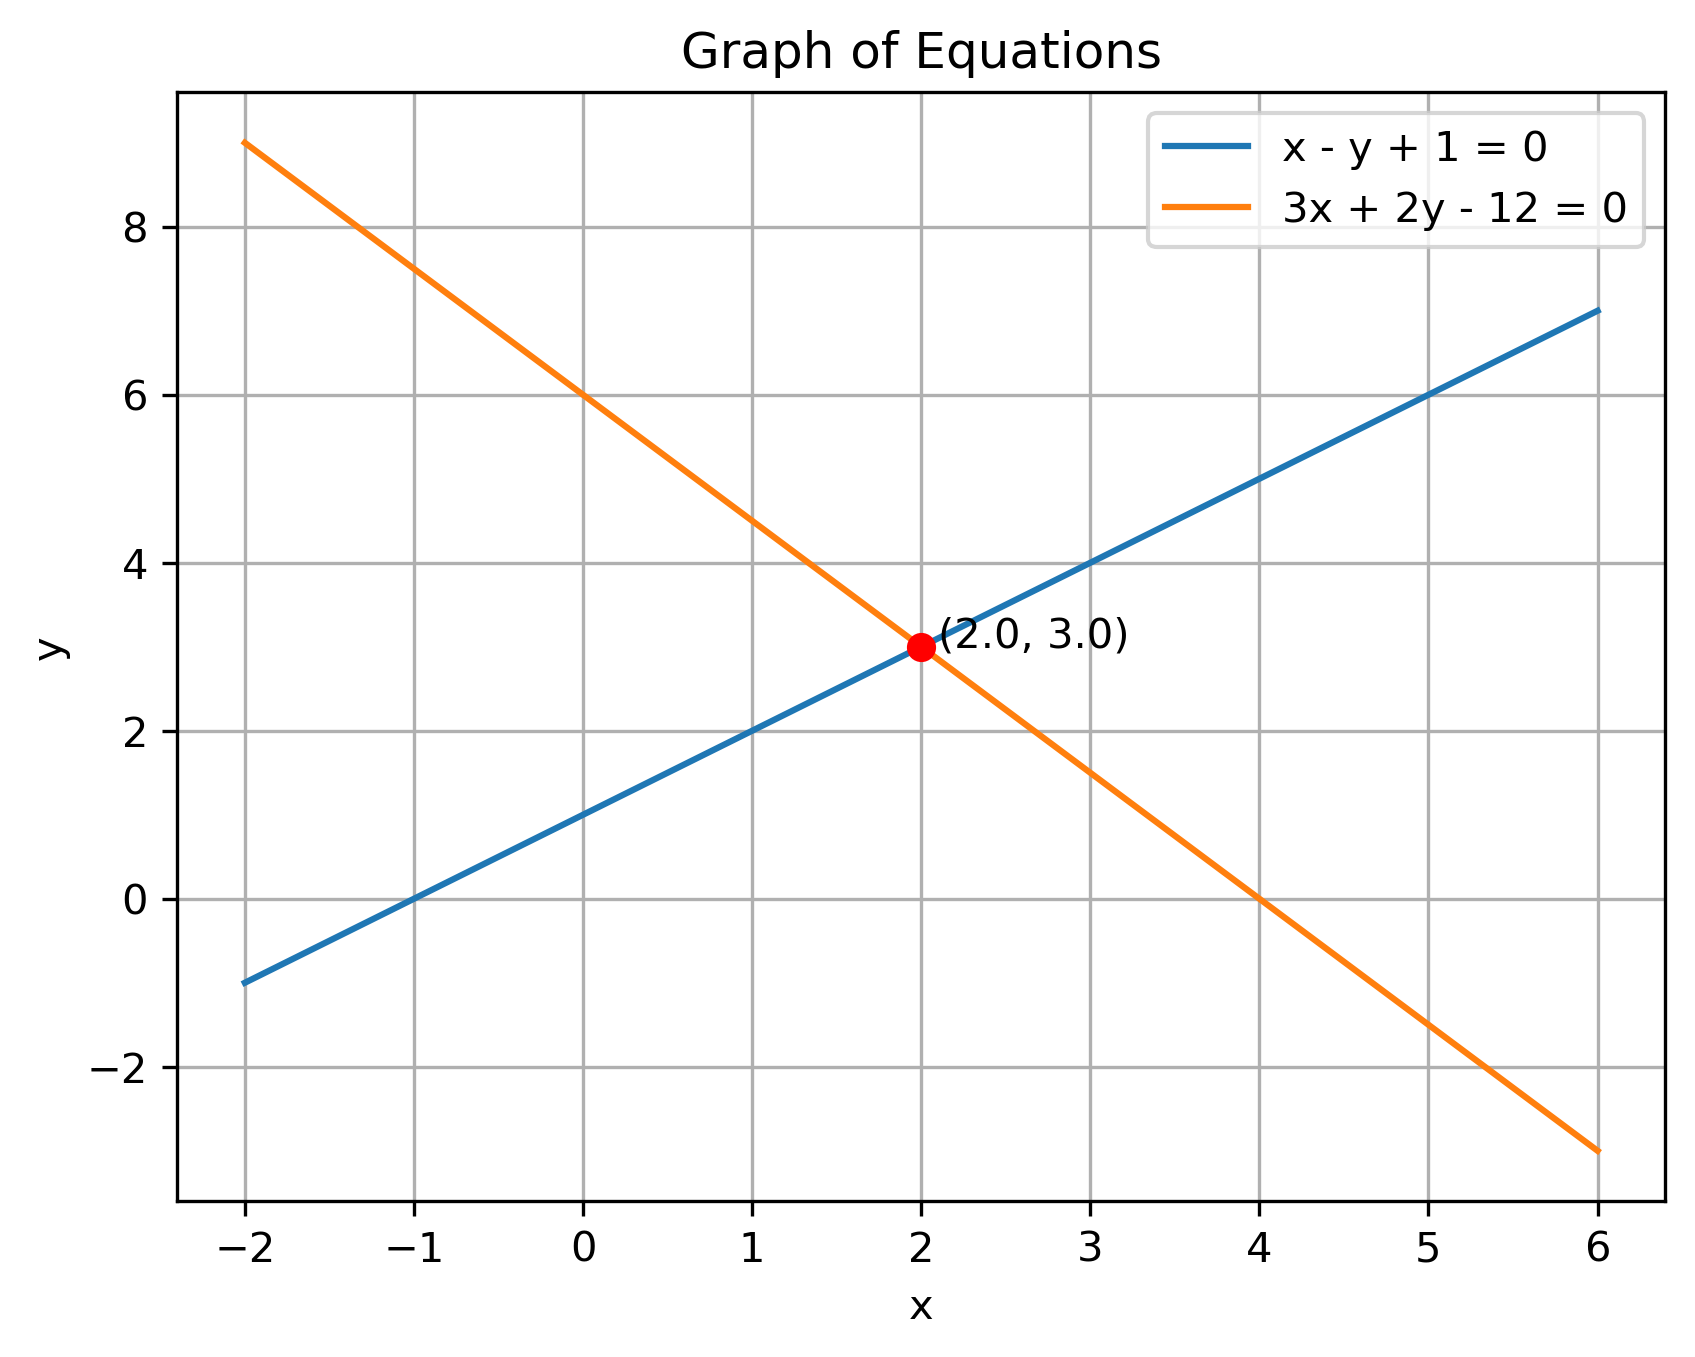
\includegraphics[width=1\linewidth]{figs/equations_solution}
		\caption{Intersection of the given lines}
		\label{fig:equationssolution}
	\end{figure}
	
\end{document}
